\section{Discussion}

For comparison of logistic regression, the figure \ref{fig:logistic-comparison} 
is borrowed from \cite{ComparisonData}.
\begin{figure}[H]
\begin{center}
    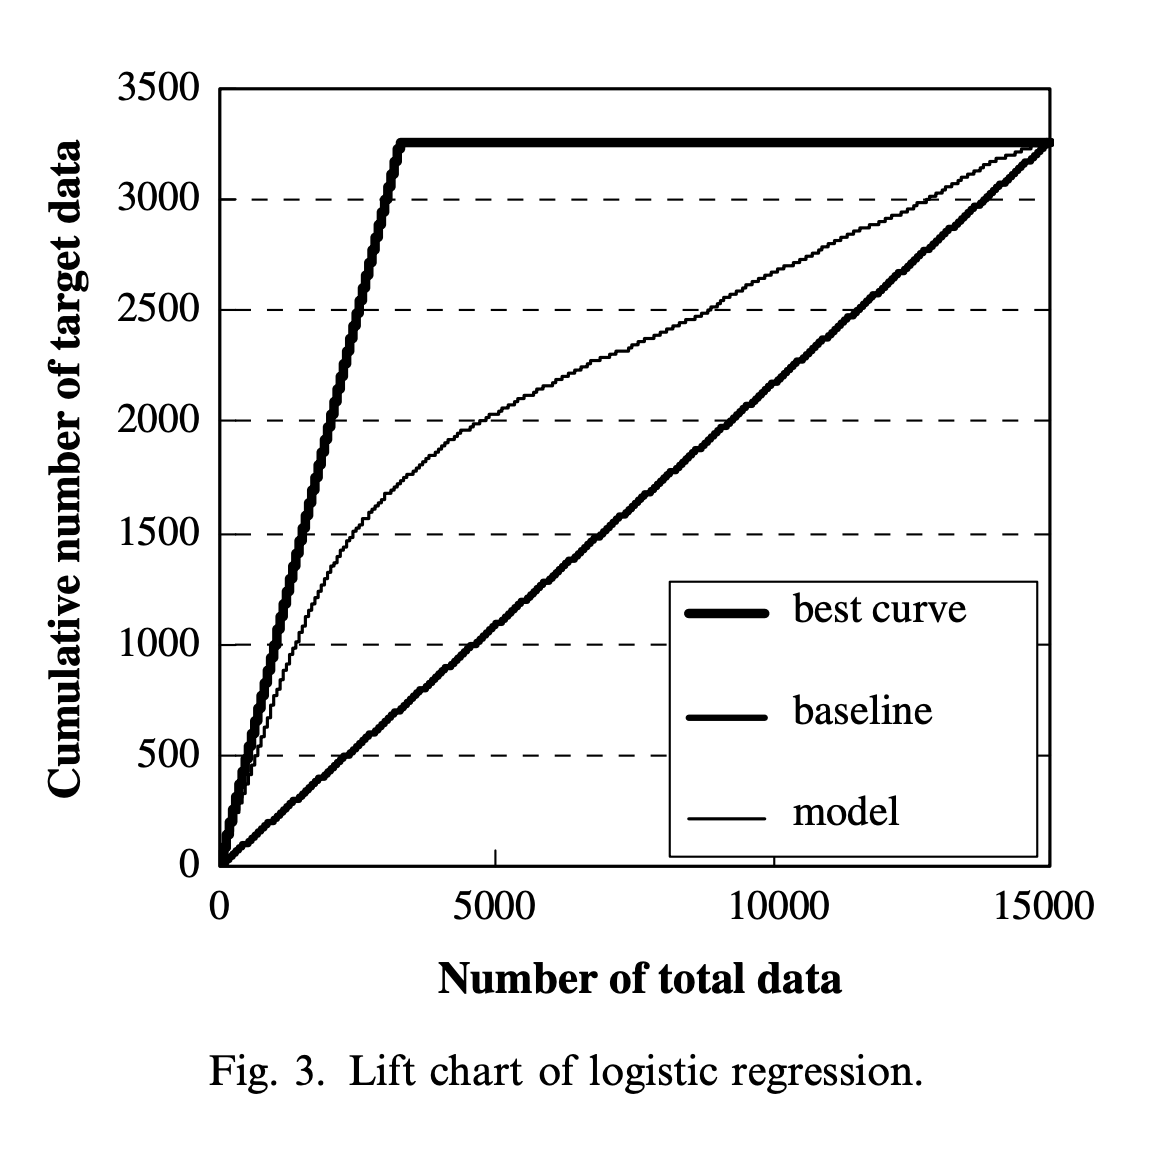
\includegraphics[width=0.7\textwidth]{figures/logistic_article.png}
\end{center}
\caption[caption]{Cumulative gain char for logistic regression in ~\cite{ComparisonData} (Figure 3)}
\label{fig:logistic-comparison}
\end{figure}

In \cite{ComparisonData}, logistic regression performs slightly better than
can be seen in figure \ref{fig:logistic-basic}. From the slightly steeper
curve of in the cumulative gain chart (\ref{fig:logistic-comparison}). 
Logistic regression is, however, ill-suited to perform well on a dataset
that is imbalanced like this one. As can be seen from figures 
\ref{fig:logistic-cumul}, \ref{fig:logistic-confmat}, \ref{fig:logistic-roc},
drastic improvement can be made. When the data is imbalanced, the logistic
algorithm classifies every input into one class, which can be seen in the
confusion matrix in figure \ref{fig:logistic-basic}(b).
The sampling methods seem to remedy this, likely because the cost-function
of the model can no longer be minimized by putting all inputs in the same class.

SMOTE reaches roughly the same performance as random over-sampling, but the
ROC curves in figure \ref{fig:logistic-roc}(a, c) shows the methods lead to
a slightly different curvature. This may be due to random-oversampling using
extra copies of the existing inputs in the miniature class, while SMOTE
synthesizes new samples that are only similar to existing ones.

ADASYN performs very well reaching a cross-validation
accuracy of ~$95\%$, but is still outclassed by the built-in balanced
weighting of scikit-learn's model, which performs perfectly, despite its
straightforward nature. It would seem then, that even though synthesizing 
more data in the minority class does improve the performance, 
this type of problem responds extremely well to weighting.

Based on the superb performance of the model with weighting, a possible 
explanation for this could be that heavier weighting of the minority
class is the most efficient way to expose which features of the inputs are
key when classifying it. It would be interesting to see if this behaviour
emerges for other datasets of a similar nature, when applying logistic
regression.

In figure \ref{fig:forest-performance}, Random Forests are applied to the
same data set. Random forests could not reach the performance of logistic
regression, but peaked with random over-sampling just around the level of the 
logistic model with ADASYN. The other sampling methods resulted in very little
improvement over no balacing effort. This may be due to lack of hyperparameter
tuning, which was not a focus of this project.
Nevertheless, 


